\chapter{Investigation of Axion-Like Particles decaying to \ttbartitle}
\label{ch:alps}

Following the results of \cref{ch:ah} including the interpretations as generic scalar or pseudoscalar bosons and \ttbar bound states, this chapter is dedicated to Axion-Like Particles decaying to \ttbar. As explained in \cref{sec:theory:alps}, the coupling structure of ALPs to top quarks is identical to those of the generic pseudoscalar A, such as e.g. in the 2HDM, if the basis for the ALP is chosen appropriately (cf. \cref{eq:theory:alplagrangian2}). The difference comes from the gluon interaction term, which is absent for the model used for A in \cref{ch:ah}, and which results in an additional diagram where the ALP is produced through a contact interaction with the gluons. 

If the coefficient \cG of the ALP-gluon interaction term in \cref{eq:theory:alplagrangian2} vanishes, the forms of the Lagrangians for ALP and A become identical, and the limits for A shown in \cref{ch:ah} can be directly recasted. This is done in \cref{sec:alps:translation}. If on the other hand $\cG \neq 0$, the kinematic distributions of the ALP will differ from those of A, and the experimental results are not easily translatable. This case is addressed in the scope of this work through an phenomenological study on simulation only. The technical setup of this study is described in \cref{sec:alps:setup}, after which the distributions of ALP and A are compared for different benchmark points in \cref{sec:alps:ALPvsA}. Projected exclusion limits for the $\cG \neq 0$ case are presented in \cref{sec:alps:limits}, and a short summary is given in \cref{sec:alps:summary}.

%\section{Introduction and definitions}

\section{Translation of experimental limits}
\label{sec:alps:translation}

In the basis of \cref{eq:theory:alplagrangian2}, the ALP Lagrangian is identical in form to the Lagrangian of the generic pseudoscalar A given in \cref{eq:theory:lag_ah} as long as the gluon interaction coefficient \cG vanishes. For this case, one finds by comparing the coefficients that the phenomenology will be identical if

\begin{equation}
    \frac{\ct}{f_a} = \frac{\gAtt}{v}
\end{equation}

\noindent where $v=\SI{246}{\GeV}$ is the SM Higgs vacuum expectation value. Thus, the experimental results of \cref{ch:ah}, particularly the limits on \gAtt presented in ??, can be recasted into limits on the ALP coupling $\ct/f_a$ for the case $\cG = 0$. This is shown in \cref{fig:alps:translation} for two different (fixed) ALP widths, similar to ??.
The observed limits are shown with and without a \ttbar bound state contribution as modeled by \etat in the background modeling, again similar to ??, and the same excess as in \cref{ch:ah} is seen for at low ALP masses when the \etat contribution is not included.
\todo{quantify excess}.

\begin{figure}[t]
    \centering
    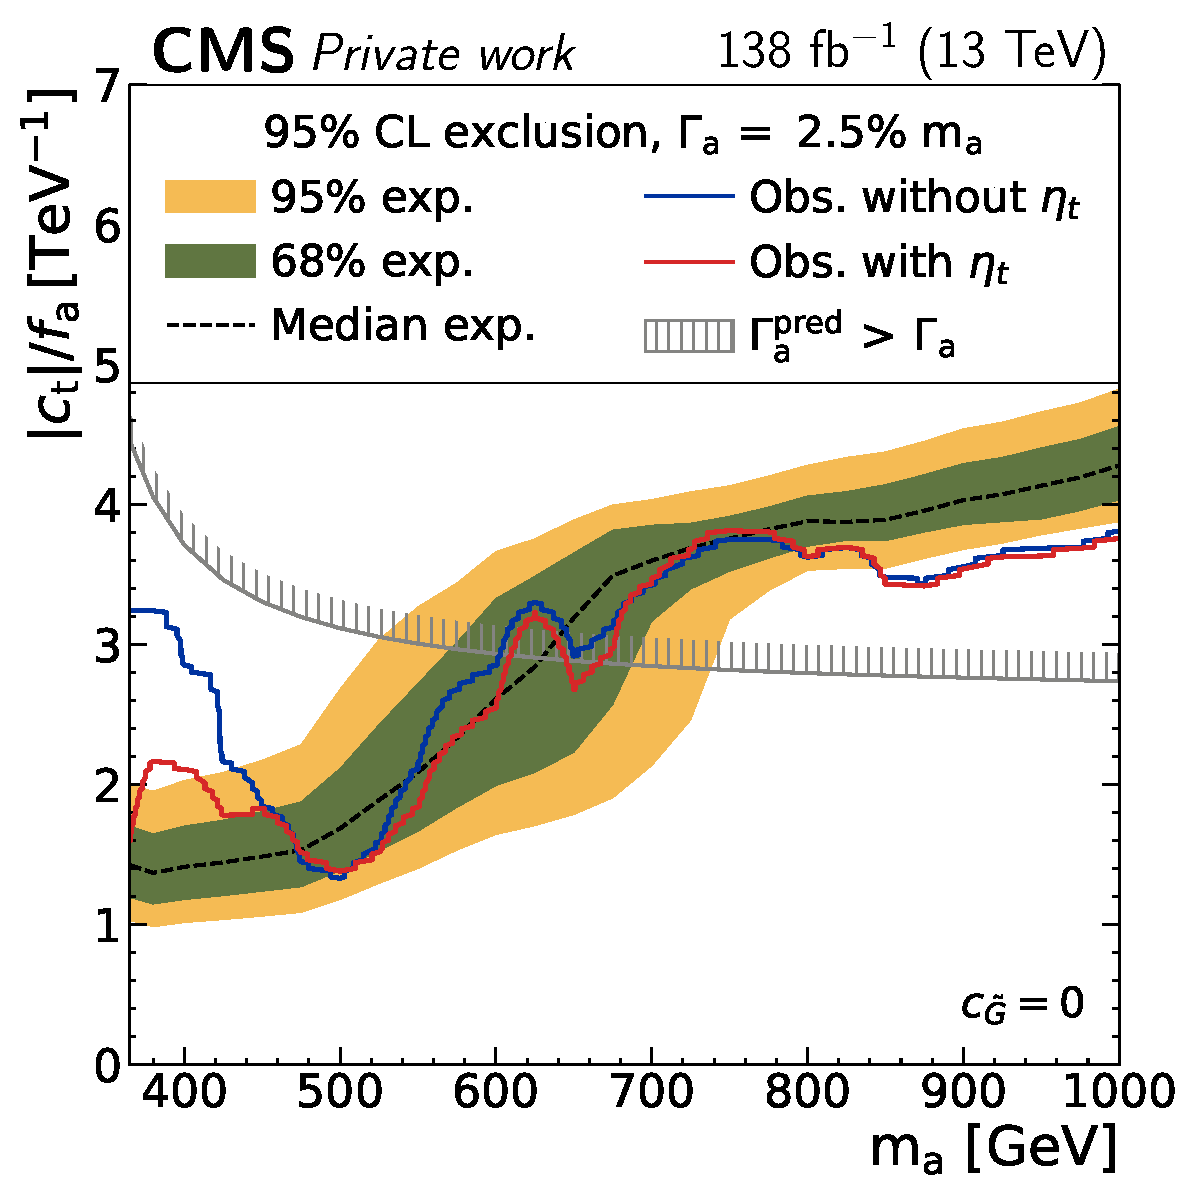
\includegraphics[width=0.49\textwidth]{figures/alps/A_limit_w2p5_g-scan_alp_lx.pdf}
    \hfill
    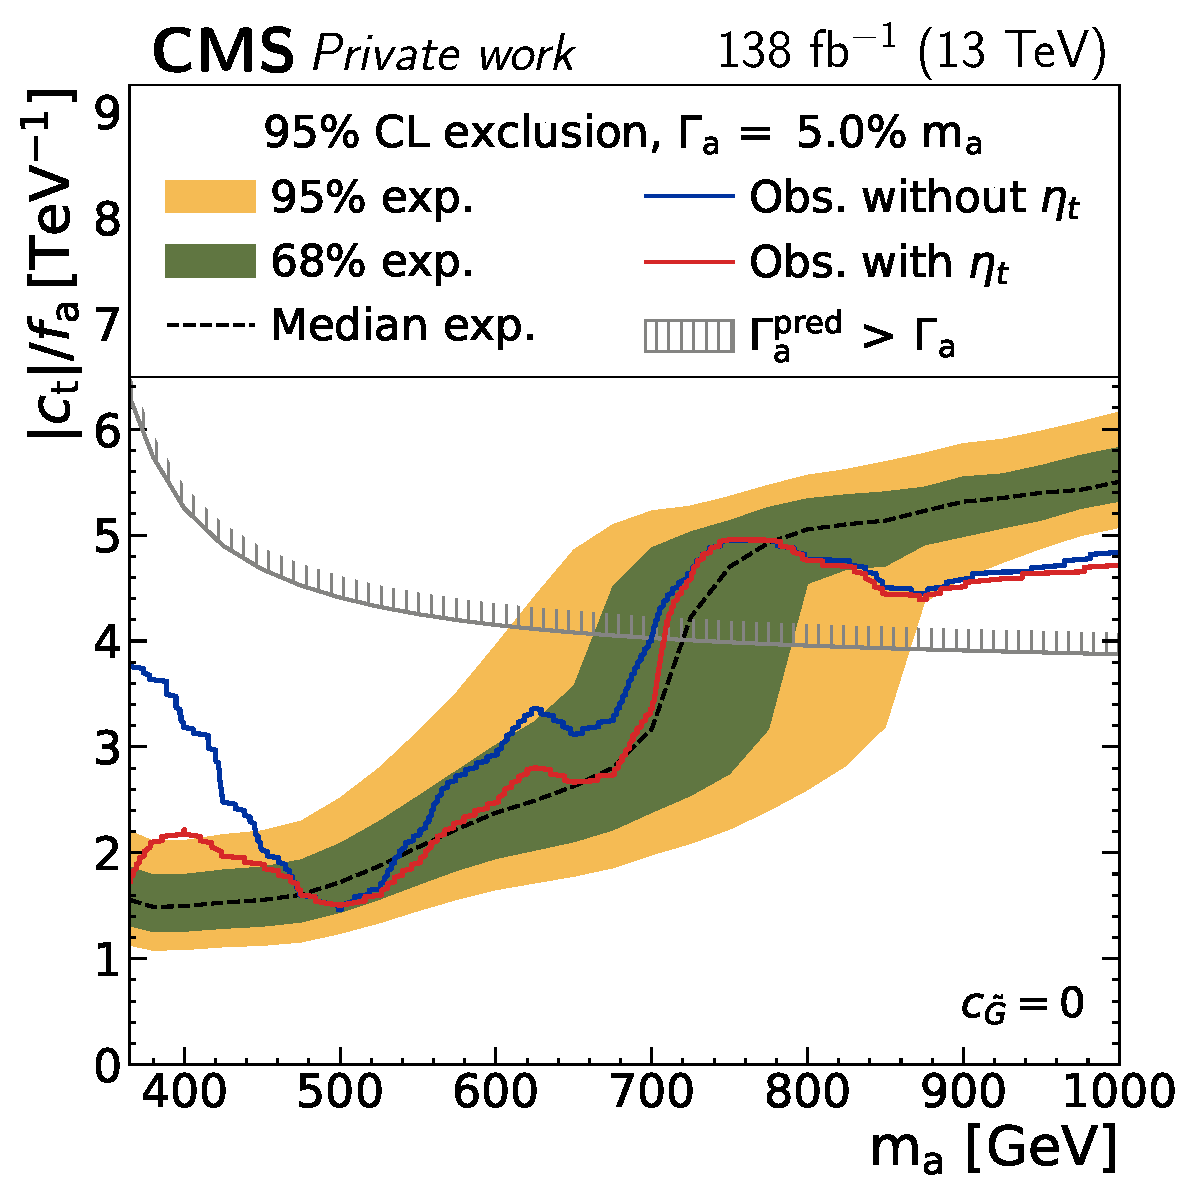
\includegraphics[width=0.49\textwidth]{figures/alps/A_limit_w5p0_g-scan_alp_lx.pdf}
    \caption{
        \textbf{ALP limits for $\cG = 0$.} Expected and observed limits on the ALP-top coupling $\ct / f_a$ as a function of the ALP mass for the case $\cG = 0$, translated from the results of \cref{ch:ah}. The expected limit (black line) is shown without contribution from \ttbar bound states in the background modeling, while the observed limit is shown both without \ttbar bound states (blue) and with \etat included in the background, same as in ?? (red).
    }
    \label{fig:alps:translation}
\end{figure}

\section{Phenomenological setup}
\label{sec:alps:setup}

The remainder of this chapter is dedicated to exploring an ALP decaying to \ttbar for the case $\cG \neq 0$, for which the results of \cref{ch:ah} are not easily translatable since the distributions are expected to differ in shape. Due to time constraints, it was not possible as part of this work to investigate this case experimentally in the same fashion as done in \cref{ch:ah}. Instead, a phenomenological study is performed on MC simulation only, using a setup that approximates the workflow in \cref{ch:ah}.

To do so, MC samples for the signal are generated at LO in QCD with \madgraph for two different ALP masses (\SI{400}{\GeV} and \SI{800}{\GeV}). For the ALP, and UFO model taken from \citere{Brivio:2017ije} is used and modified to include the top quark loop form factor including finite mass effects, according to the expressions given in \citere{Bonilla:2021ufe}. Both possible production diagrams, as shown in \cref{fig:theory:ggALP}, as well as their interference with the SM are considered. A similar ME reweighting technique as in \cref{sec:ah:mereweighting} is used to obtain samples for different widths and \cG values. For the generic pseudoscalar A as well as the SM \ttbar background, the same generators as in \cref{sec:ah:datasets} are used (\madgraph and \powhegvtwo \hvq, respectively). For all samples, the NNPDF~3.1 PDF set~\cite{NNPDF:2017mvq} is used, and \pythia 8.2 is used to simulate initial and final state radiation~\cite{Pythia:2015}.

Only the dilepton decay channel of \ttbar is considered, and no detector simulation is performed. Instead, the truth-level top quarks and leptons after parton showering are used, and a Gaussian smearing is applied to \mtt randomly on a per-event basis, the standard deviation of which is chosen so that the resolution of the resulting distribution matches that observed in full detector simulation. Since this study was performed before the results of \cref{ch:ah} were public, its predecessor \citere{CMS:HIG-17-027} is used to extract the resolution by fitting to the \mtt distributions displayed therein. The result is $\sigma(\mtt) / \mtt = 15\%$, which is somewhat lower than the widths found using the full detector simulation in \cref{sec:ah:kinreco} (c.f. \cref{fig:ah:resolution}). However, it should be cautioned that since the true \mtt smearing in the full detector simulation is not perfectly Gaussian, the results are not one-to-one comparable. 

The experimental acceptance and efficiency, defined as the fraction of $\ttbar \rightarrow \ell\ell$ ($\ell$ being electrons, muons or leptonically decaying taus) events to survive all trigger and selection requirements, is estimated to be $10.6\%$ for both signal and \ttbar background, also based on \citere{CMS:HIG-17-027}. This is similar to the observations in \cref{ch:ah} \todo{add numbers}.

Since the ALP always has a CP-odd coupling to top quarks (cf. \cref{eq:theory:alplagrangian2}), it is expected to decay to a \ttbar system in the \term{1}{S}{0} state, identically to A. This is true irrespective of the gluon coupling \cG since it only affects the production, not the decay, and the ALP as a colorless, spinless particle has no internal degrees of freedom. Thus, \mtt and \chel are good discriminating variables, again similar to A, while \chan (optimal for CP-even couplings) does not offer much additional discrimination and is not considered here. For simplicity, instead of a multi-dimensional binning in \mtt and \chel like in \cref{ch:ah}, a one-dimensional binning in \mtt only is used, and events are required to have $\chel > 0.6$ to enhance the ALP signal over the background.

A simplified version of the likelihood model from \cref{ch:ah} is used, implemented in \texttt{pyhf}~\cite{pyhf_joss}. Only sources of systematic uncertainty arising from theory are considered, namely:

\begin{itemize}
    \item Missing higher orders in the matrix element, estimated from varying renormalization and factorization scale by factors of 2,
    \item The PDF uncertainty, estimated as the envelope of 100 pseudo-Hessian NNPDF~3.1 replicas~\cite{NNPDF:2017mvq},
    \item The total \ttbar background production cross section, taken as a log-normal uncertainty of $6\%$ following \citere{CMS:HIG-17-027},
    \item The top quark mass in the \ttbar background, varied in the range $\mt = 172.5 \pm 1 \, \si{\GeV}$.
\end{itemize}

Of these, like in the experimental result, the top quark mass is the most important especially for ALPs with masses close to the \ttbar threshold. \todo{somehow introduce three different scenarios for systs.}

\section{Comparison of ALP and A}
\label{sec:alps:ALPvsA}

\begin{figure}
    \centering
    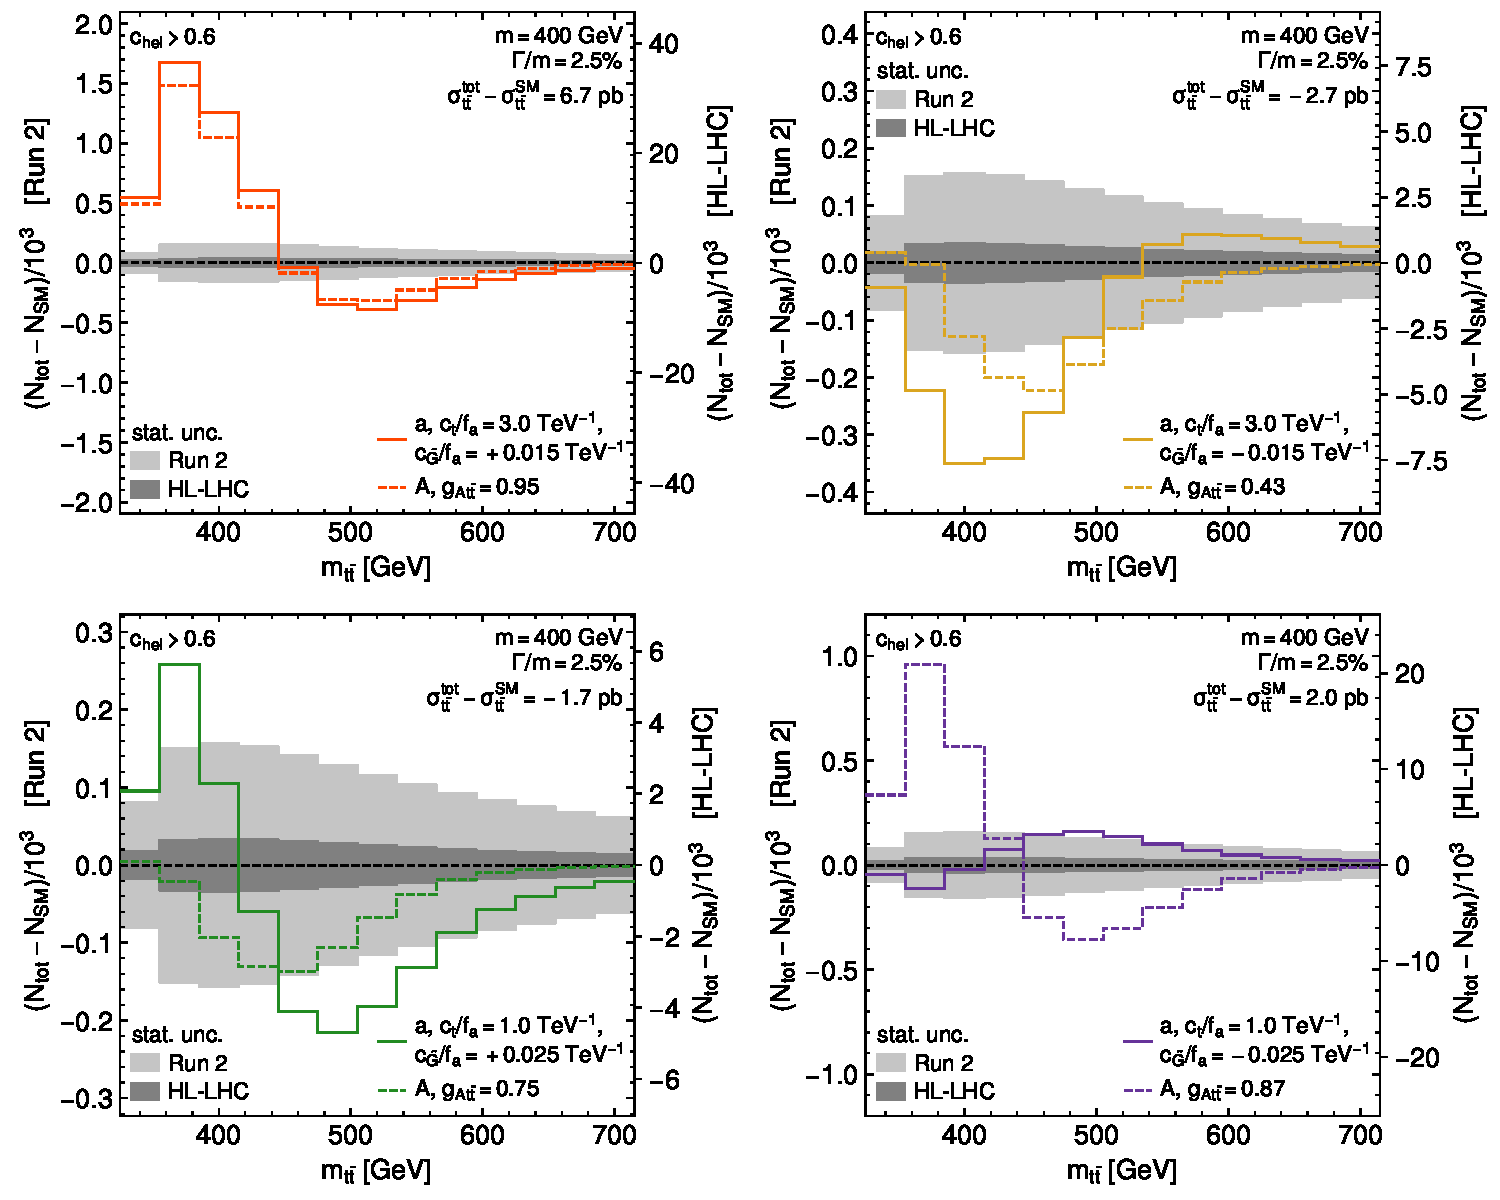
\includegraphics[width=0.99\linewidth]{figures/alps/mttplots.pdf}
    \caption{\textbf{Expected \mtt distributions for $pp \rightarrow a/A \rightarrow \ttbar$.} Shown are both ALP and A at a mass of \SI{400}{\GeV} for four benchmark points, with the SM subtracted. The couplings for A and a are adjusted such that the inclusive cross section is identical. The grey bands show the expected statistical uncertainty for Run~2 and HL-LHC.}
    \label{fig:alps:mttplots}
\end{figure}

\section{Projected limits for ALPs}
\label{sec:alps:limits}

\begin{figure}[t]
    \centering
    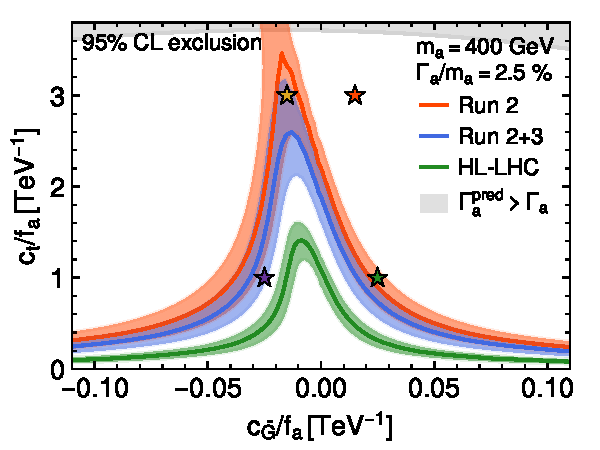
\includegraphics[width=0.49\textwidth]{figures/alps/limits_m400_w2p5_notmass_small_width.pdf}
    \hfill
    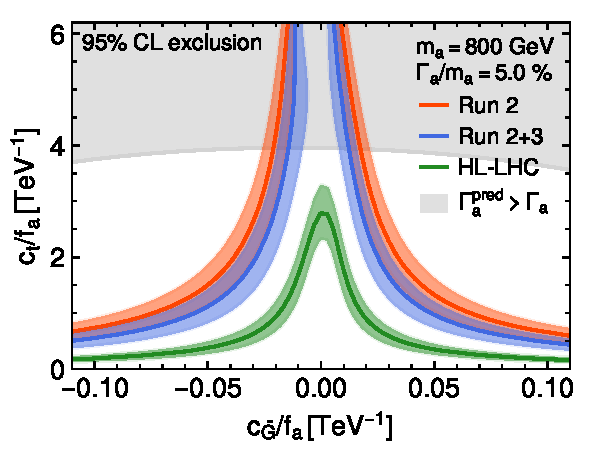
\includegraphics[width=0.49\textwidth]{figures/alps/limits_m800_w5p0_notmass_small.pdf}
    \caption{
        \textbf{Projected ALP limits.} Projected 95\% exclusion limits in the plane of $\cG/f_a$ and $\ct/f_a$ for a mass of \SI{400}{\GeV} and a width of 2.5\% (left) as well as \SI{800}{\GeV} and 5.0\% (right). The limits are shown for three different integrated luminosities, corresponding to Run~2, Run~2+3, and the HL-LHC.
    }
    \label{fig:alps:limits}
\end{figure}

\begin{figure}[t]
    \centering
    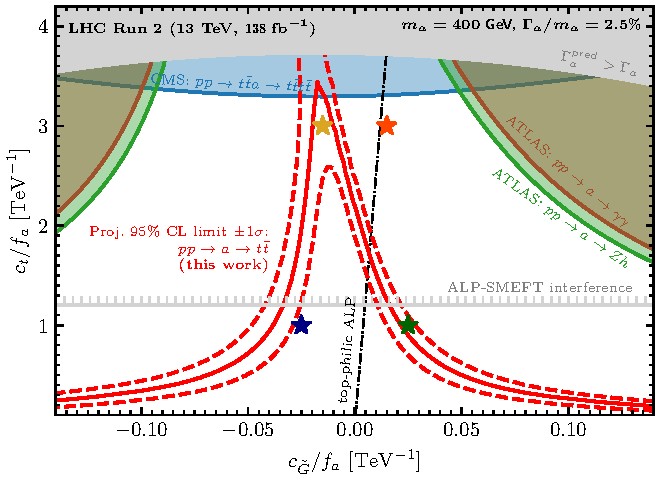
\includegraphics[width=0.8\textwidth]{figures/alps/sum400.pdf}
    \caption{
        \textbf{Comparison of limits from different search channels.} 95\% exclusion limits in the plane of $\cG/f_a$ and $\ct/f_a$ for a mass of \SI{400}{\GeV} and a width of 2.5\% (left) from different search channels. The projected limits from this work are overlaid in red.
    }
    \label{fig:alps:summary}
\end{figure}

\section{Summary}
\label{sec:alps:summary}